\newpage
\section{Badania operatorów}

\subsection{Wybrane ćwiczenia}
\label{sec:wybrane-cwiczenia}
Dla każdego z wybranych do automatycznej oceny zadań w tabeli \ref{tab:ocena-funkcje}, w trakcie szkolenia wykonuje się ćwiczenie które ma na celu opanowanie tej umiejętności. Plan prób do zrealizowania podczas badania doborem ćwiczeń ma naśladować program szkolenia praktycznego operatora BSP. Dzięki temu będzie możliwe zaobserwowanie procesu uczenia się pilotażu, oraz opisanie za pomocą liczb jak dokładnie przebiega dla bardziej i mniej doświadczonych kursantów.

Zgodnie z wymogami przytoczonymi w rozdziale \ref{sec:tradycyjny-egzamin}, zawis wykonywany jest w określonym miejscu w kilku orientacjach BSP względem operatora. W doświadczeniach autora instruktor określa miejsce zawisu poprzez znak na ziemi lub umieszczenie niewielkiego obiektu, przykładowo pachołka drogowego. Ćwiczenie rozpoczyna się od zawisu tyłem do operatora --- czyli przód BSP pokrywa się z kierunkiem patrzenia. Wtedy sterowanie jest najłatwiejsze, ponieważ pochylenie i przechylenie BSP odbywa się w tę samą stronę jak wychylenie drążka sterowania. Po wybranym przez siebie czasie, instruktor określa kolejny kierunek w którym należy zwrócić przód BSP. Oprócz tego ćwiczy się zachowanie stałej wysokości, jednak często nie jest określone jaka musi być dokładnie. Z tego powodu w ramach tego ćwiczenia, jako wzorcową wartość wysokości przyjmowana jest ta którą miał BSP kiedy po raz pierwszy znalazł się w poziomej odległości $ 0.5 \text{m} $ od wyznaczonego miejsca.

Kolejnym wykonywanym ćwiczeniem może być przelot po obwodzie kwadratu, utrzymując przód w kierunku ruchu. Sprawdza umiejętność lotu po prostej w czterech różnych orientacjach BSP. Narożniki kwadratu mogą być oznaczone podobnie jak miejsce wykonywania zawisu. Podobnie jak inne szczegóły szkolenia i egzaminu, długość boku tego kwadratu powinna być dostosowana do statku powietrznego. Na podstawie doświadczenia autora, dla wielowirnikowca średniej wielkości tj. masie startowej 3~kg zostanie wykorzystany kwadrat o boku 8~m. Umiejscowienie operatora nie jest szczególnie ważne, dopóki znajduje się w bezpiecznej odległości od oblatywanego obszaru. Oczekiwane jest, że wykona ćwiczenie nie przemieszczając się za BSP. Poglądowy schemat ilustrujący to ćwiczenie zamieszczono na rysunku \ref{fig:kwadrat}.

\begin{figure}[!h]
    \centering 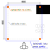
\includegraphics[width=0.6\linewidth]{kwadrat.pdf}
    \caption{Schemat ćwiczenia lotu wzdłuż prostych}
    \label{fig:kwadrat}
\end{figure}

Umiejętności wprowadzenia w zakręt, krążenia, oraz wyprowadzenia z zakrętu według doświadczeń autora są rozwijane w ramach wykonywania jednego ćwiczenia. W przeciwieństwie do manewrów opisywanych do tej pory, w tym przypadku wymagana jest pewna prędkość postępowa. Lot po okręgu wymaga wytworzenia przyspieszenia dośrodkowego o wartości proporcjonalnej do prędkości lotu. Wymagając pewnej minimalnej prędkości, utrzymanie przodu BSP w kierunku ruchu wymaga wtedy odpowiedniego przechylenie wielowirnikowca do środka zakrętu. Z tego powodu ćwiczenie rozpoczyna się od rozpędzenia w wybranym kierunku. Następnie wykonywany jest zakręt, lot wokół okręgu, wyjście z zakrętu i wyhamowanie do zawisu. Zwraca się głównie uwagę na zakreślenie równomiernego koła wokół obszaru wykonywania ćwiczeń, oraz zachowanie dynamicznego charakteru manewru. Dla stosowanego modelu wielowirnikowca arbitralnie dobrano promień koła 5~m, który po sprawdzeniu w symulacji przez autora został uznany za adekwatny. Wzajemne położenie trasy przelotu i naziemnych oznaczeń w widoku z góry ilustruje rysunek \ref{fig:kolo}.

\begin{figure}[!h]
    \centering 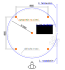
\includegraphics[width=0.8\linewidth]{kolo.pdf}
    \caption{Schemat ćwiczenia lotu w zakręcie po okręgu}
    \label{fig:kolo}
\end{figure}

\subsubsection{Implementacja w aplikacji}
Zgodnie z założeniami poczynionymi na etapie projektowania aplikacji wizualnej, dla każdego ćwiczenia przygotowano osobną scenę, w nomenklaturze silnika Unreal Engine nazywaną ,,mapą''. Aby oznaczyć miejsce zawisu umieszczono pachołek drogowy o wysokości 600~mm w odległości 7~m od operatora. Bezpośrednio nad nim znajduje się niewidoczny w trakcie ćwiczenia prostopadłościan, na rysunku \ref{fig:examhover} reprezentowany zielonymi liniami. Wlot BSP do tego obszaru rozpoczyna ocenę, zapisuje obecną wysokość jako referencyjną i rozpoczyna pomiar czasu. Niebieski znacznik orientacji umieszczony pomiędzy miejscem zawisu a operatorem wskazuje kierunek w którym należy skierować przód statku powietrznego. Po upływie 10 sekund od wejścia w zawis nad pachołkiem, ocena jest zatrzymywana, a znacznik obracany o 90°. Operator ma 10 sekund na odchylenie w nowym kierunku, po czym ocena jest wznawiana. Rozpoczęcie oceny każdorazowo jest sygnalizowane krótkim dźwiękiem. Taki cykl jest wykonywany cztery razy, dla kolejnych kursów różniących się o 90°.

\begin{figure}[!h]
    \centering \includegraphics[width=\linewidth]{examhover.png}
    \caption{Zrzut ekranu obszaru do wykonywania zawisu}
    \label{fig:examhover}
\end{figure}

Kolejne wykonywane ćwiczenie ma na celu opanowanie lotu po prostej. Identyczne pachołki drogowe jak dla oznaczenia miejsca zawisu zostały rozmieszczone w sposób opisany na rysunku \ref{fig:kwadrat}. Na wysokości 2~m nad ziemią ułożono trasę składającą się z czterech odcinków łączących kolejne wierzchołki kwadratu. Ponieważ ćwiczenie rozpoczyna się i kończy w tym samym miejscu, na każdym narożniku dodano bramki kontrolne, na rysunku \ref{fig:examsquare} widoczne jako półprzezroczyste niebieskie koła o średnicy 2~m. Poprawne ukończenie zadania wymaga przelotu przez każdą z nich. Aby czytelniej przekazać przebieg trasy, na początku ćwiczenia widoczna jest tylko bramka startu. W momencie gdy BSP znajdzie się w pobliżu przeciwległego narożnika trasy, start jest ukrywany, a zamiast tego włączana jest czerwona bramka końca.

\begin{figure}[!h]
    \centering \includegraphics[width=\linewidth]{examsquare.png}
    \caption{Zrzut ekranu obszaru do lotu po obwodzie kwadratu}
    \label{fig:examsquare}
\end{figure}

Ćwiczenie lotu w zakręcie zostało zaimplementowane w sposób bardzo zbliżony do lotu wzdłuż obwodu kwadratu. Wytyczono okrąg o średnicy i położeniu zgodnym z rysunkiem \ref{fig:kolo}. Ponieważ ćwiczenie wykonywane jest z większą prędkością, a mniejszą precyzją, podczas szkolenia praktycznego często odbywa się nieco wyżej niż pozostałe. Aby to odwzorować, trasa znajduje się na wysokości 4~m nad terenem, a bramki mają średnicę 3~m. Wygląd mapy w edytorze przedstawia rysunek \ref{fig:examcircle}. Także w tym przypadku, podczas lotu początkowo widoczna jest tylko bramka oznaczająca początek próby, a po przeleceniu połowy trasy tylko bramka końcowa.

\begin{figure}[!h]
    \centering \includegraphics[width=\linewidth]{examcircle.png}
    \caption{Zrzut ekranu obszaru do lotu w zakręcie}
    \label{fig:examcircle}
\end{figure}

\subsection{Konfiguracja systemu}
We wszystkich próbach wykorzystywany był domyślny model dynamiczny wielowirnikowca zaimplementowany w bibliotece ArduPilot SITL \cite{sitl-model}. Najważniejsze parametry modelu przedstawiono w tabeli \ref{tab:sitl-model}. Należy zwrócić uwagę, że ponieważ modelowana jest jedna konfiguracja elektrycznego statku powietrznego, masa pozostaje stała --- nie ma potrzeby rozdzielać jej na maksymalną, suchą etc.

\begin{table}[!h] \centering
    \caption{Charakterystyczne wielkości modelowanego BSP}
    \label{tab:sitl-model}

    \begin{tabular}{|l | r|l |}
    \hline
    Cecha charakterystyczna & Wielkość & Jednostka \\ \hline \hline
    Masa & 3 & kg \\ \hline
    Moment bezwładności w osi $ X $ & 0,0230 & $ \text{kg}\cdot\text{m}^2 $ \\ \hline
    Moment bezwładności w osi $ Y $ & 0,0230 & $ \text{kg}\cdot\text{m}^2 $ \\ \hline
    Moment bezwładności w osi $ Z $ & 0,0459 & $ \text{kg}\cdot\text{m}^2 $ \\ \hline
    Konfiguracja & \multicolumn{2}{c|}{\emph{quadrotor X}} \\ \hline
    Długość & 600 & mm \\ \hline
    Szerokość & 600 & mm \\ \hline
    Średnica śmigła & 350 & mm \\ \hline
    Liczba śmigieł & 4 & szt. \\ \hline
    Rozstaw śmigieł & 250 & mm \\ \hline
    Moc pobierana w zawisie & 354 & W \\ \hline
  \end{tabular}
\end{table}

Operatorzy sterowali modelem wykorzystując rzeczywisty nadajnik zdalnego sterowania \emph{FrSKY Horus X10 Express} widoczny na rysunku \ref{fig:frsky-horus}. Drążki sterowe były ustawione w układzie \emph{Mode 2}, który jest najbardziej popularny \cite{mcnabb2021}. Lewy drążek wychylany w lewo lub prawo powodował odpowiadające sterowanie w osi odchylenia. Wychylenie lewego drążka do góry zwiększa wysokość, a w dół obniża lot. Prawy drążek sterowy ma przypisane osie pochylenia i przechylenia identycznie jak w samolotach. Trzy osie, z wyjątkiem sterowania wysokością są wyposażone w sprężyny które przywracają je do położenia centralnego. Większość lotów została wykonana z wizualizacją w okularach Oculus Rift, z dwoma wyjątkami. Loty operatora Charlie oraz loty według kamery zamontowanej na BSP zostały wykonane na podstawie obrazu na płaskim monitorze komputerowym.

\begin{figure}[!h]
    \centering \includegraphics[width=0.8\linewidth]{frsky-horus.jpg}
    \caption{Wykorzystywany nadajnik zdalnego sterowania}
    \label{fig:frsky-horus}
\end{figure}

\subsection{Przebieg eksperymentu}

\subsubsection{Uczestnicy}
Uczestnicy eksperymentu wyrazili chęć ukrycia ich tożsamości w niniejszej pracy. Z tego powodu do uczestników zostały przypisane kolejne litery alfabetu. Aby uniknąć pomyłki z symbolem matematycznym zastosowanym w innej części pracy, w danych eksperymentalnych oraz opracowaniach wyników są oznaczeni wyrazami z alfabetu radiotelefonicznego ICAO. Stosowane formy męskie czasowników wynikają z gramatycznego rodzaju słowa ,,operator'', nie są powiązane z płcią uczestników. Doświadczenie poszczególnych uczestników jest przedstawione w niniejszym rozdziale, jako informacja użyteczna w analizie uzyskanych wyników.

Podsumowując, w grupie znalazło się trzech uczestników bez żadnego doświadczenia w pilotażu BSP oraz czterech którzy wcześniej wykonywali loty. Spośród uczestników z doświadczeniem, wszyscy wykonywali wcześniej loty wielowirnikowcami. Dwóch z nich posiada świadectwo kwalifikacji.

Operator Alfa nie miał wcześniej doświadczenia związanego z pilotażem BSP. Jako jedyny zgłosił, że regularnie gra w gry komputerowe.

Operator Bravo przed badaniem kilkukrotnie wykonywał loty BSP typu wielowirnikowiec wyposażonym w układ autopilota, każdorazowo wykorzystując automatyczną stabilizację pozycji opartą o system GNSS. Ostatnie loty wykonywał ponad 12 miesięcy przed badaniem.

Operator Charlie nie miał wcześniej doświadczenia związanego z pilotażem BSP. Jako jedyny nie wykonywał lotów w okularach VR.

Operator Delta nie miał wcześniej doświadczenia związanego z pilotażem BSP.

Operator Echo przed badaniem wykonywał loty BSP typu wielowirnikowiec wyposażonym w układ autopilota, każdorazowo wykorzystując automatyczną stabilizację pozycji opartą o system GNSS. Uzyskał uprawnienia BVLOS w kategorii szczególnej. Ostatnie loty wykonywał ponad 4 miesiące przed badaniem.

Operator Foxtrot przed badaniem kilkukrotnie wykonywał loty BSP typu wielowirnikowiec wyposażonym w układ autopilota, każdorazowo wykorzystując automatyczną stabilizację pozycji opartą o system GNSS. Ostatnie loty wykonywał w miesiącu badania.

Operator Golf (autor pracy) przed badaniem wykonywał loty BSP różnych typów, z układami autopilota oraz bez żadnej automatycznej stabilizacji. Ostatnie loty wykonywał ponad 2 miesiące przed badaniem. Jako jedyny korzystał z utworzonego systemu przed przeprowadzeniem badania. Wpływ doświadczenia zdobytego w systemie został zminimalizowany, przez sprawdzanie funkcjonalności bez podłączania symulacji AP~SITL. Poza badaniem wykorzystywano trywialny model kinematyczny, w którym naciśnięcie przycisku na klawiaturze komputera powodowało przemieszczanie symulowanego BSP ze stałą prędkością.

\subsubsection{Wykonane loty}
Pierwotnie przygotowany plan zadań do wykonania w trakcie badania musiał zostać zmodyfikowany, aby dostosować go do umiejętności uczestników. Według doświadczenia autora, podczas tradycyjnego szkolenia nauka zawisu bez automatycznej stabilizacji pozycji zajmuje około kilkudziesięciu minut. Niestety, czas który uczestnicy mogli poświęcić na badania był bardzo ograniczony. Różniąca się liczba lotów wynika głównie z tego czynnika. W tabeli \ref{tab:loty} zebrano wszystkie loty zapisane w trakcie badania, z których będą wybierane odpowiednie podzbiory w opracowaniu wyników.

\begin{table}[!h] \centering
    \caption{Podsumowanie wszystkich lotów zebranych w trakcie badań}
    \label{tab:loty}
    \renewcommand{\arraystretch}{1.3} % Wyższe o 30% rzędy tabeli

    \begin{tabular}{| l *{7}{| c} |}
        \hline
        \textbf{Rodzaj lotu} &
        \spheading[5em]{Alfa} &
        \spheading[5em]{Bravo} &
        \spheading[5em]{Charlie} &
        \spheading[5em]{Delta} &
        \spheading[5em]{Echo} &
        \spheading[5em]{Foxtrot} &
        \spheading[5em]{Golf} \\ \hline \hline
        Zawis z GNSS               & 1 & 1 & 1 & 2 & 1 &   & 1 \\ \hline
        Zawis bez GNSS, bez wiatru & 2 & 1 & 1 & 1 & 1 &   & 2 \\ \hline
        Zawis bez GNSS, z wiatrem  & 6 & 6 & 2 &   & 5 &   & 6 \\ \hline
        j. w., przerwana próba     &   &   & 2 & 4 & 1 & 2 &   \\ \hline
        Kwadrat z GNSS             & 6 & 6 &   & 1 & 1 &   &   \\ \hline
        Koło z GNSS                & 4 &   &   &   &   &   & 3 \\ \hline
        Koło z GNSS, widok FPV     & 2 &   &   &   &   &   & 2 \\ \hline
    \end{tabular}
\end{table}

Opisane w tabeli rodzaje lotów były wykonywane z różnymi ustawieniami autopilota. W lotach oznaczonych ,,z GNSS'' był aktywny tryb \emph{LOITER}, w którym autopilot utrzymuje ostatnio zadaną pozycję poziomą. Wychylenie prawego drążka sterowego należy interpretować jako \emph{position command}, czyli przemieszczanie punktu w którym sterownik ma utrzymywać statek powietrzny. Wszyscy operatorzy deklarowali, że wpływ wiatru w tym trybie jest niezauważalny. Podczas lotów opisanych ,,bez GNSS'' autopilot pracował w trybie \emph{ALT\_HOLD}, w którym nie jest zachowywane stałe położenie. Wychylenie prawego drążka jest odczytywane jako \emph{attitude command}, czyli powoduje pochylenie i przechylenie BSP. W przeciwieństwie do trybu \emph{LOITER}, po puszczeniu sterownic BSP wróci do położenia poziomego, ale będzie się przemieszczał z dotychczasową prędkością z przyspieszeniem wynikającym z wiatru i siły oporów aerodynamicznych. Wysokość oraz kąt odchylenia w obu trybach były utrzymywane automatycznie, operator miał możliwość sterować w obu tych osiach za pomocą lewego drążka sterowego.

We wszystkich ćwiczeniach w których występował wiatr, wiał z prędkością $ 2 \frac{\text{m}}{\text{s}} $ stałą niezależnie od położenia i czasu. Wyłączono turbulencje oraz efekt przyziemny, powodujący zwiększanie się prędkości wiatru wraz ze zwiększaniem wysokości nad podłożem. W trakcie jednego lotu kierunek pozostawał stały, ale był zmieniany pomiędzy kolejnymi podejściami do tego samego ćwiczenia. Ponieważ zawis jest wykonywany w czterech orientacjach, a operatorzy określali kompensację ukośnego kierunku wiatru jako trudniejszą, zastosowano algorytm tworzący serię niewymiernych, niepowtarzających się kątów. W pierwszej kolejności kąt pełny jest dzielony na dwie części według zasady złotego podziału, a do następnych obliczeń zapisywany jest mniejszy z tak otrzymanych kątów. Tę wartość opisano w równaniu \ref{eq:zlotypodzial} literą $ \alpha $. Przemieszczając się wzdłuż obwodu koła o ten kąt, uzyska się najbardziej niewymierny rozkład punktów na okręgu \cite{ridley1982}. Na pierwszy kierunek wiatru przyjęto 180°, czyli zza pleców operatora. Spośród czterech kierunków kardynalnych ten wybrano na najłatwiejszy, ponieważ dryfujący BSP pozostaje w polu widzenia. Zbiór kierunków wiatru które wykorzystano przy wykonanej ilości prób przedstawiono na rysunku \ref{fig:wiatr}.

\begin{align}
    \label{eq:zlotypodzial}
    \begin{cases}
        \frac{\alpha}{\beta} = \frac{\beta}{360^{\circ}} \\
        \alpha + \beta = 360^{\circ}
    \end{cases} \Rightarrow \frac{\beta}{\alpha} = \phi &\approx 1.61803\dots
    \\
    \alpha &\approx 137.508^{\circ}
\end{align}

\begin{figure}[!h]
    \centering 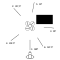
\includegraphics[width=0.6\linewidth]{wiatr.pdf}
    \caption{Kierunki wiatru wykorzystywane w próbach zawisu}
    \label{fig:wiatr}
\end{figure}

Próby były przerywane w przypadku gdy uczestnik po oddaleniu się BSP na znaczną odległość, deklarował że nie jest w stanie powrócić do miejsca wykonywania ćwiczenia. Ćwiczenie lotu po okręgu wymagało najbardziej złożonej nawigacji w porównaniu do pozostałych dwóch. Podczas podejść w widoku FPV obserwowano wizualizację z kamery przemieszczającej się razem z BSP, tworząc wrażenie podobne do siedzenia w kokpicie załogowego statku powietrznego.

Wynikiem każdej z prób jest plik tekstowy w formacie CSV zawierający wszystkie zebrane dane. Nadajnik operatora wykorzystywany w próbie jest bezpośrednio połączony z symulacją BSP. Następnie stan symulacji jest przesyłany protokołem MAVLink do wizualizacji i wyświetlany na okularach operatora. Położenie, orientacja przestrzenna, prędkość statku powietrznego oraz odległość od trasy referencyjnej są zapisywane dla każdej wyświetlonej klatki obrazu oraz wysyłane do oceny. Serwer oceny oblicza poszczególne składowe błędu, oraz odsyła wiadomość z wynikami do aplikacji wizualnej. Wyniki oceny są przypisywane do odpowiedniego stanu na podstawie znacznika czasu, dzięki czemu mogą być zapisane w tym samym wierszu pliku z wynikami. Dalsza obróbka danych może być zrealizowana w dowolnym pakiecie obliczeniowym. Z powodu znacznej liczby plików, w niniejszej pracy wykorzystano \cite{soft:pandas} do analizy wyników i przygotowania wykresów.

\subsection{Wyniki}
Zadanie zawisu na wietrze, bez stabilizacji pozycji zostało wykonane przez wszystkich uczestników badania. Poziom trudności tego zadania spowodował największą różnicę w wynikach. Zebrane oceny przedstawiono w tabeli \ref{tab:oceny}. Należy zwrócić uwagę, że zgodnie z definicjami w tabeli \ref{tab:ocena-funkcje} lepszy lot oznacza niższą wartość oceny. Te same dane rozdzielone na ocenę pozycji oraz kąta odchylenia przedstawia wykres na rysunku \ref{fig:plot-ocena}. Zgodnie z definicją funkcji oceny, każdy operator wykonywał to zadanie przez ten sam okres czasu. Próby które zostały przerwane przez utratę kontroli nie spełniały tego warunku, dlatego nie została dla nich obliczona ocena.

\begin{table}[!h] \centering
    \caption{Oceny przypisane operatorom w zawisie na wietrze}
    \label{tab:oceny}
    \renewcommand{\arraystretch}{1.3} % Wyższe o 30% rzędy tabeli

    \begin{tabular}{| r *{8}{| c } |}
        \hline
        \textbf{Kolejne podejście} &
        \spheading[5em]{Alfa} &
        \spheading[5em]{Bravo} &
        \spheading[5em]{Charlie} &
        \spheading[5em]{Delta} &
        \spheading[5em]{Echo} &
        \spheading[5em]{Foxtrot} &
        \spheading[5em]{Golf} \\ \hline \hline
        1                &  44.41 & 23.41 &   P   & P &   P   & P & 1.87 \\ \hline
        2                & 100.92 & 25.48 & 77.72 & P & 25.08 & P & 2.52 \\ \hline
        3                &  23.43 & 26.90 & 67.72 & P & 34.78 &   & 1.26 \\ \hline
        4                &  12.41 & 15.20 &   P   & P & 48.60 &   & 3.91 \\ \hline
        5                &  53.31 & 35.76 &       &   & 12.89 &   & 2.26 \\ \hline
        6                &  44.46 & 25.07 &       &   & 74.11 &   & 3.91 \\ \hline\hline
        \textbf{średnia} &  46.49 & 25.30 & 72.72 &   & 39.09 &   & 2.62 \\ \hline
    \end{tabular}
\end{table}

\begin{figure}[!h]
    \centering \includegraphics[width=\linewidth]{plot-ocena.pdf}
    \caption{Wykres ocen operatorów rozdzielony na składowe}
    \label{fig:plot-ocena}
\end{figure}

Na podstawie dokonanej oceny można wysunąć kilka wniosków. Nie sprawdziła się hipoteza stawiana w podrozdziale \ref{sec:wybrane-cwiczenia}, że wyniki uczestników będą coraz lepsze wraz z kolejnymi podejściami. Prawdopodobnie wynika to z niewielkiej ilości doświadczenia które zdobyli w trakcie badań. Próby były wykonywane bezpośrednio po sobie, po wczytaniu zadania z nowym kierunkiem wiatru uczestnicy mieli się zaznajomić z warunkami i rozpocząć oceniany manewr kiedy będą gotowi.

Można zaobserwować zbieżność przyznanej oceny z poziomem doświadczenia uczestników badania. Na potrzeby tego porównania, każdej przerwanej próbie zostanie przypisany najgorszy wynik osiągnięty w ukończonym ćwiczeniu, czyli $ 100.92 $. Po takim poszerzeniu dostępnych danych, grupa operatorów Alfa, Charlie i Delta którzy po raz pierwszy pilotowali BSP osiągali średni wynik $ 73.56 $. Operatorzy Bravo, Echo i Foxtrot którzy mieli doświadczenie z BSP, ale brak ćwiczenia w sterowaniu ręcznym, średnio uzyskali znacząco lepszy wynik $ 43.46 $. Niestety tylko operator Golf miał wcześniejsze doświadczenia w ręcznym pilotowaniu. Skrajnie mała próbka uniemożliwia jednoznaczną identyfikację czynników które spowodowały że średnia ocena wyniosła tylko $ 2.622 $.

Jak można zaobserwować na wykresie \ref{fig:plot-ocena} znacznie większe różnice pomiędzy operatorami były widoczne w zakresie sterowania położeniem BSP. Poza kilkoma gorszymi podejściami, sterowanie w kanale odchylenia było wykonywane bardzo poprawnie. Kolejne orientacje w których należało wykonywać zawis różniły się od siebie o 90°. Na histogramie przedstawionym na rysunku \ref{fig:plot-yaw-histogram} widać że oprócz malejącej częstotliwości dla większych wartości błędu, widać lokalne maksimum w okolicach właśnie 90°. Najprawdopodobniej odpowiada to sytuacjom w których operator nie wykonał obrotu w trakcie przeznaczonego na to czasu.

\begin{figure}[!h]
    \centering \includegraphics[width=0.8\linewidth]{plot-yaw-histogram.pdf}
    \caption{Histogram wartości błędu w osi odchylenia}
    \label{fig:plot-yaw-histogram}
\end{figure}

Aby lepiej przedstawić rozkład błędu w następujących rozważaniach zostanie wykorzystany wykres pudełkowy\footnote{ang. \emph{box-plot}}. Dla każdego zestawu próbek jest rysowany prostokąt, którego dolna i górna granica oznaczają odpowiednio pierwszy i trzeci kwartyl wartości. Pozioma linia wewnątrz prostokąta jest umieszczona na wysokości mediany. Odcinki na zewnątrz prostokąta zwane ,,wąsami'', w tej pracy zawsze oznaczają 2 oraz 98 centyl. Z powodu dużej ilości próbek podlegających ocenie, elementy odstające nie są rysowane ponieważ znacznie pogarszały czytelność.

Na rysunku \ref{fig:plot-operator-pos-box} przedstawiono wartości błędu położenia BSP w kolejnych klatkach symulacji, tj. próbkowane z częstotliwością 45~Hz. Zostały wybrane ze wszystkich ukończonych prób zawisu przy wietrze, oraz pogrupowane według operatorów. Można zaobserwować że mediana dla wszystkich serii oprócz Golf znajduje się na bardzo podobnym poziomie: $ 2.88 \pm 0.13 \text{m} $, ale różnią się górną granicą. Fakt że przypisano im znacznie różniące się oceny, wskazuje na osiągnięcie celu penalizowania dużych błędów wskazanego w rozdziale \ref{sec:dobor-kryteriow}.

\begin{figure}[!h]
    \centering \includegraphics[width=0.8\linewidth]{plot-operator-pos-box.pdf}
    \caption{Charakterystyka błędu pozycji według operatorów}
    \label{fig:plot-operator-pos-box}
\end{figure}

Oprócz porównania między sobą poszczególnych operatorów, zbadano wpływ różnych warunków na trudność wykonywania manewru zawisu. Jak widać na wykresie \ref{fig:plot-wind-pos-box}, kierunek wiatru nie miał dużego wpływu na wyniki, chociaż potwierdziła się teza, że wiatr wprost za pleców będzie najłatwiejszy do skompensowania.

\begin{figure}[!h]
    \centering \includegraphics[width=0.8\linewidth]{plot-wind-pos-box.pdf}
    \caption{Charakterystyka błędu pozycji względem wiatru}
    \label{fig:plot-wind-pos-box}
\end{figure}

Podczas badań operatorzy wielokrotnie komentowali, że zawis w orientacjach innych niż przodem BSP w kierunku patrzenia jest znacznie trudniejszy, w szczególności przodem do operatora. Stany lotu pogrupowano według najbliższej wielokrotności 90° w osi odchylenia, a wyniki przedstawiono na rysunku \ref{fig:plot-orientation-pos-box}. Wartości błędu potwierdzają że zawis przodem BSP ,,od siebie'' faktycznie jest najłatwiejszy, ale w przeciwieństwie do subiektywnych opinii nie widać znaczącej różnicy w pozycji odwróconej.

\begin{figure}[!h]
    \centering \includegraphics[width=0.8\linewidth]{plot-orientation-pos-box.pdf}
    \caption{Charakterystyka błędu pozycji względem orientacji BSP}
    \label{fig:plot-orientation-pos-box}
\end{figure}

Zdecydowanie czynnikiem najsilniej wpływającym na trudność utrzymania pozycji jest konieczność prowadzenia stałych poprawek. W przypadku stabilizacji pozycji na podstawie wskazań symulowanego GNSS, operatorzy musieli jedynie dolecieć w odpowiednim miejsce, a następnie obracać w osi odchylenia zgodnie z poleceniami. Zawis bez GNSS w bezwietrznym powietrzu wymaga samodzielnego zatrzymania BSP w odpowiednim punkcie, sterując w zasadzie przyspieszeniem w kierunku poziomym. Po wytraceniu całej prędkości nad znacznikiem, wystarcza obracanie i okazjonalne korekty.

Ręczne sterowanie pochyleniem i przechyleniem przy wietrze jest znacznie większym obciążeniem dla operatora. Konieczne są ciągłe poprawki w celu utrzymania BSP w jednym miejscu. Zachowanie stałej prędkości wymaga znalezienia takiego wychylenia drążka sterowego żeby pozioma składowa siły ciągu równoważyła napór wiatru. Ponadto po każdej zmianie orientacji BSP, równowaga jest osiągnięta przy innym położeniu sterownicy. Na wykresie \ref{fig:plot-task-pos-box} wyraźnie widać pogarszające się wyniki wraz z rosnącą ilością poprawek wymaganych od operatora.

\begin{figure}[!h]
    \centering \includegraphics[width=0.8\linewidth]{plot-task-pos-box.pdf}
    \caption{Charakterystyka błędu pozycji względem stabilizacji wymaganej od operatora}
    \label{fig:plot-task-pos-box}
\end{figure}

Ostatnim czynnikiem którego wpływ sprawdzono, jest perspektywa z której operator obserwuje położenie BSP względem zadanej ścieżki. Dane przedstawione na wykresie \ref{fig:plot-fpv-pos-box} jako jedyne w tym podrozdziale zostały zebrane w trakcie lotu po okręgu. Można zaobserwować że prowadzenie statku powietrznego jest łatwiejsze na podstawie widoku z wnętrza, ale nie jest to tak duża różnica jak przewidywano.

\begin{figure}[!h]
    \centering \includegraphics[width=0.8\linewidth]{plot-fpv-pos-box.pdf}
    \caption{Charakterystyka błędu pozycji względem perspektywy obserwacji}
    \label{fig:plot-fpv-pos-box}
\end{figure}
